
% The environment used here (theappendices) is a wrapper for the basic appendices environment which changes the appearance of the title page and the structure and appearance of the appendices in the table of contents and PDF bookmarks. The original functionality can be restored by simply removing the 'the' from the \begin{} and \end{} statements below.

\begin{theappendices}

% \chapter{Language Editing Certification}
% \centering

% This is to certify that the undersigned has reviewed and went through all the pages of the Bachelor of Science in Computer Science thesis manuscript titled \\

% \textbf{"THEMESYNC:A GRAPH-BASED DESIGN ORCHESTRATION FRAMEWORK WITH REAL-TIME CONSTRAINT SATISFACTION AND STATEFUL REFINEMENT"} \\


% of \textbf{AuthorName1}, \textbf{AuthorName2}, \textbf{AuthorName3}, as against the set of structural rules that govern research writing in accord with the composition of sentences, phrases, and words in the English language.
%  \newline \newline \newline \\

% \noindent \textbf{JUAN DE LA CRUZ} \\
% \textit{Language Editor} \\

% Date:\_\_\_\_\_\_\_\_\_\_\_\_\_\_\_\_\_\_\_\_\_\_\_


% \chapter{Secretary's Certification}
% \centering

% This is to certify that the undersigned has provided accurate recommendations, suggestions, and comments unanimously agreed and approved by the panel of examiners during the oral examination of the thesis titled \\ \textbf{"ENTER YOUR TITLE HERE"} \\  prepared and submitted by \textbf{AuthorName1}, \textbf{AuthorName2}, \textbf{AuthorName3}, and that the same have not been amended, modified or obliterated. \newline \newline \newline \\



% \textbf{MS. MARIA DAISY R. BELARDO} \\
% \textit{Secretary} \\


% Date:\_\_\_\_\_\_\_\_\_\_\_\_\_\_\_\_\_\_\_\_\_\_\_

% \chapter{JOINT AFFIDAVIT OF UNDERTAKING (Plagiarism)}

% \centering

% \textbf{JOINT AFFIDAVIT OF UNDERTAKING}


% IN WITNESS WHEREOF, I have hereunto set my name this ____ day of ___________ 202__ in
% ___________________________________, Philippines.
% SUBSCRIBED AND SWORN TO before me this ___ day of ________ at _______________, Philippines,
% affiants exhibiting to me their competent proofs of identity above stated.
% Doc. No. ___________:
% Page No.: __________:
% Book No.: __________:
% Series of 202_.


\chapter{Preprocessed CGL-Dataset Node Array for GNN Ingestion}
\label{annex:cgl-node-array}
\begin{lstlisting}
{
  "extracted_nodes": [
    {
      "semantic_category": "logo",
      "bbox": [106, 22, 284, 65]
    },
    {
      "semantic_category": "text",
      "bbox": [61, 140, 393, 67]
    }
  ],
  "extracted_color_centroids": [[135, 192, 167], [255, 128, 128]],
  "extracted_saliency_weight": 0.45
}
\end{lstlisting}

\chapter{Dynamic Content Payload for real-time runtime orchestration}
\label{annex:dynamic-content-payload}
\begin{lstlisting}
{
    "domain_context": "academic_certificate",
    "target_aspect_ratio": "4:3",
    "variable_schema": {
        "{{Institution_Logo}}": {
            "structural_class": "image_node",
            "spatial_hierarchy": 0,
            "lock_aspect_ratio": true
        },
        "{{Issuing_Organization}}": {
            "structural_class": "text_node",
            "spatial_hierarchy": 1,
            "max_characters": 150
        },
        "{{Certificate_Title}}": {
            "structural_class": "text_node",
            "spatial_hierarchy": 2,
            "max_characters": 80
        },
        "{{Presentation_Line}}": {
            "structural_class": "text_node",
            "spatial_hierarchy": 3,
            "max_characters": 60
        },
        "{{Student_Name}}": {
            "structural_class": "text_node",
            "spatial_hierarchy": 4,
            "max_characters": 80
        },
        "{{Citation_Body}}": {
            "structural_class": "text_node",
            "spatial_hierarchy": 5,
            "max_characters": 300
        },
        "{{Date_Issued}}": {
            "structural_class": "text_node",
            "spatial_hierarchy": 6,
            "max_characters": 60
        },
        "{{Certificate_ID}}": {
            "structural_class": "text_node",
            "spatial_hierarchy": 7,
            "max_characters": 40
        },
        "{{Signature_Blocks}}": {
            "structural_class": "repeating_group",
            "spatial_hierarchy": 8,
            "instantiation_count": 3
        }
    }
}
\end{lstlisting}

\chapter{Sample Annotated Master Layouts From the Empirical Dataset}
\label{annex:empirical-samples}

The empirical dataset held 200 event posters (160 for training, 40 for validation), annotated in Roboflow with four classes. \ref{fig:empirical-samples} shows six of them, and \ref{tab:empirical-counts} counts the annotated boxes by class.

% Let the figure and the table share this page (Appendix C is the document's last part).
\renewcommand{\topfraction}{0.95}
\renewcommand{\bottomfraction}{0.95}
\renewcommand{\textfraction}{0.05}
\setcounter{totalnumber}{4}
\begin{figure}[!ht]
    \centering
    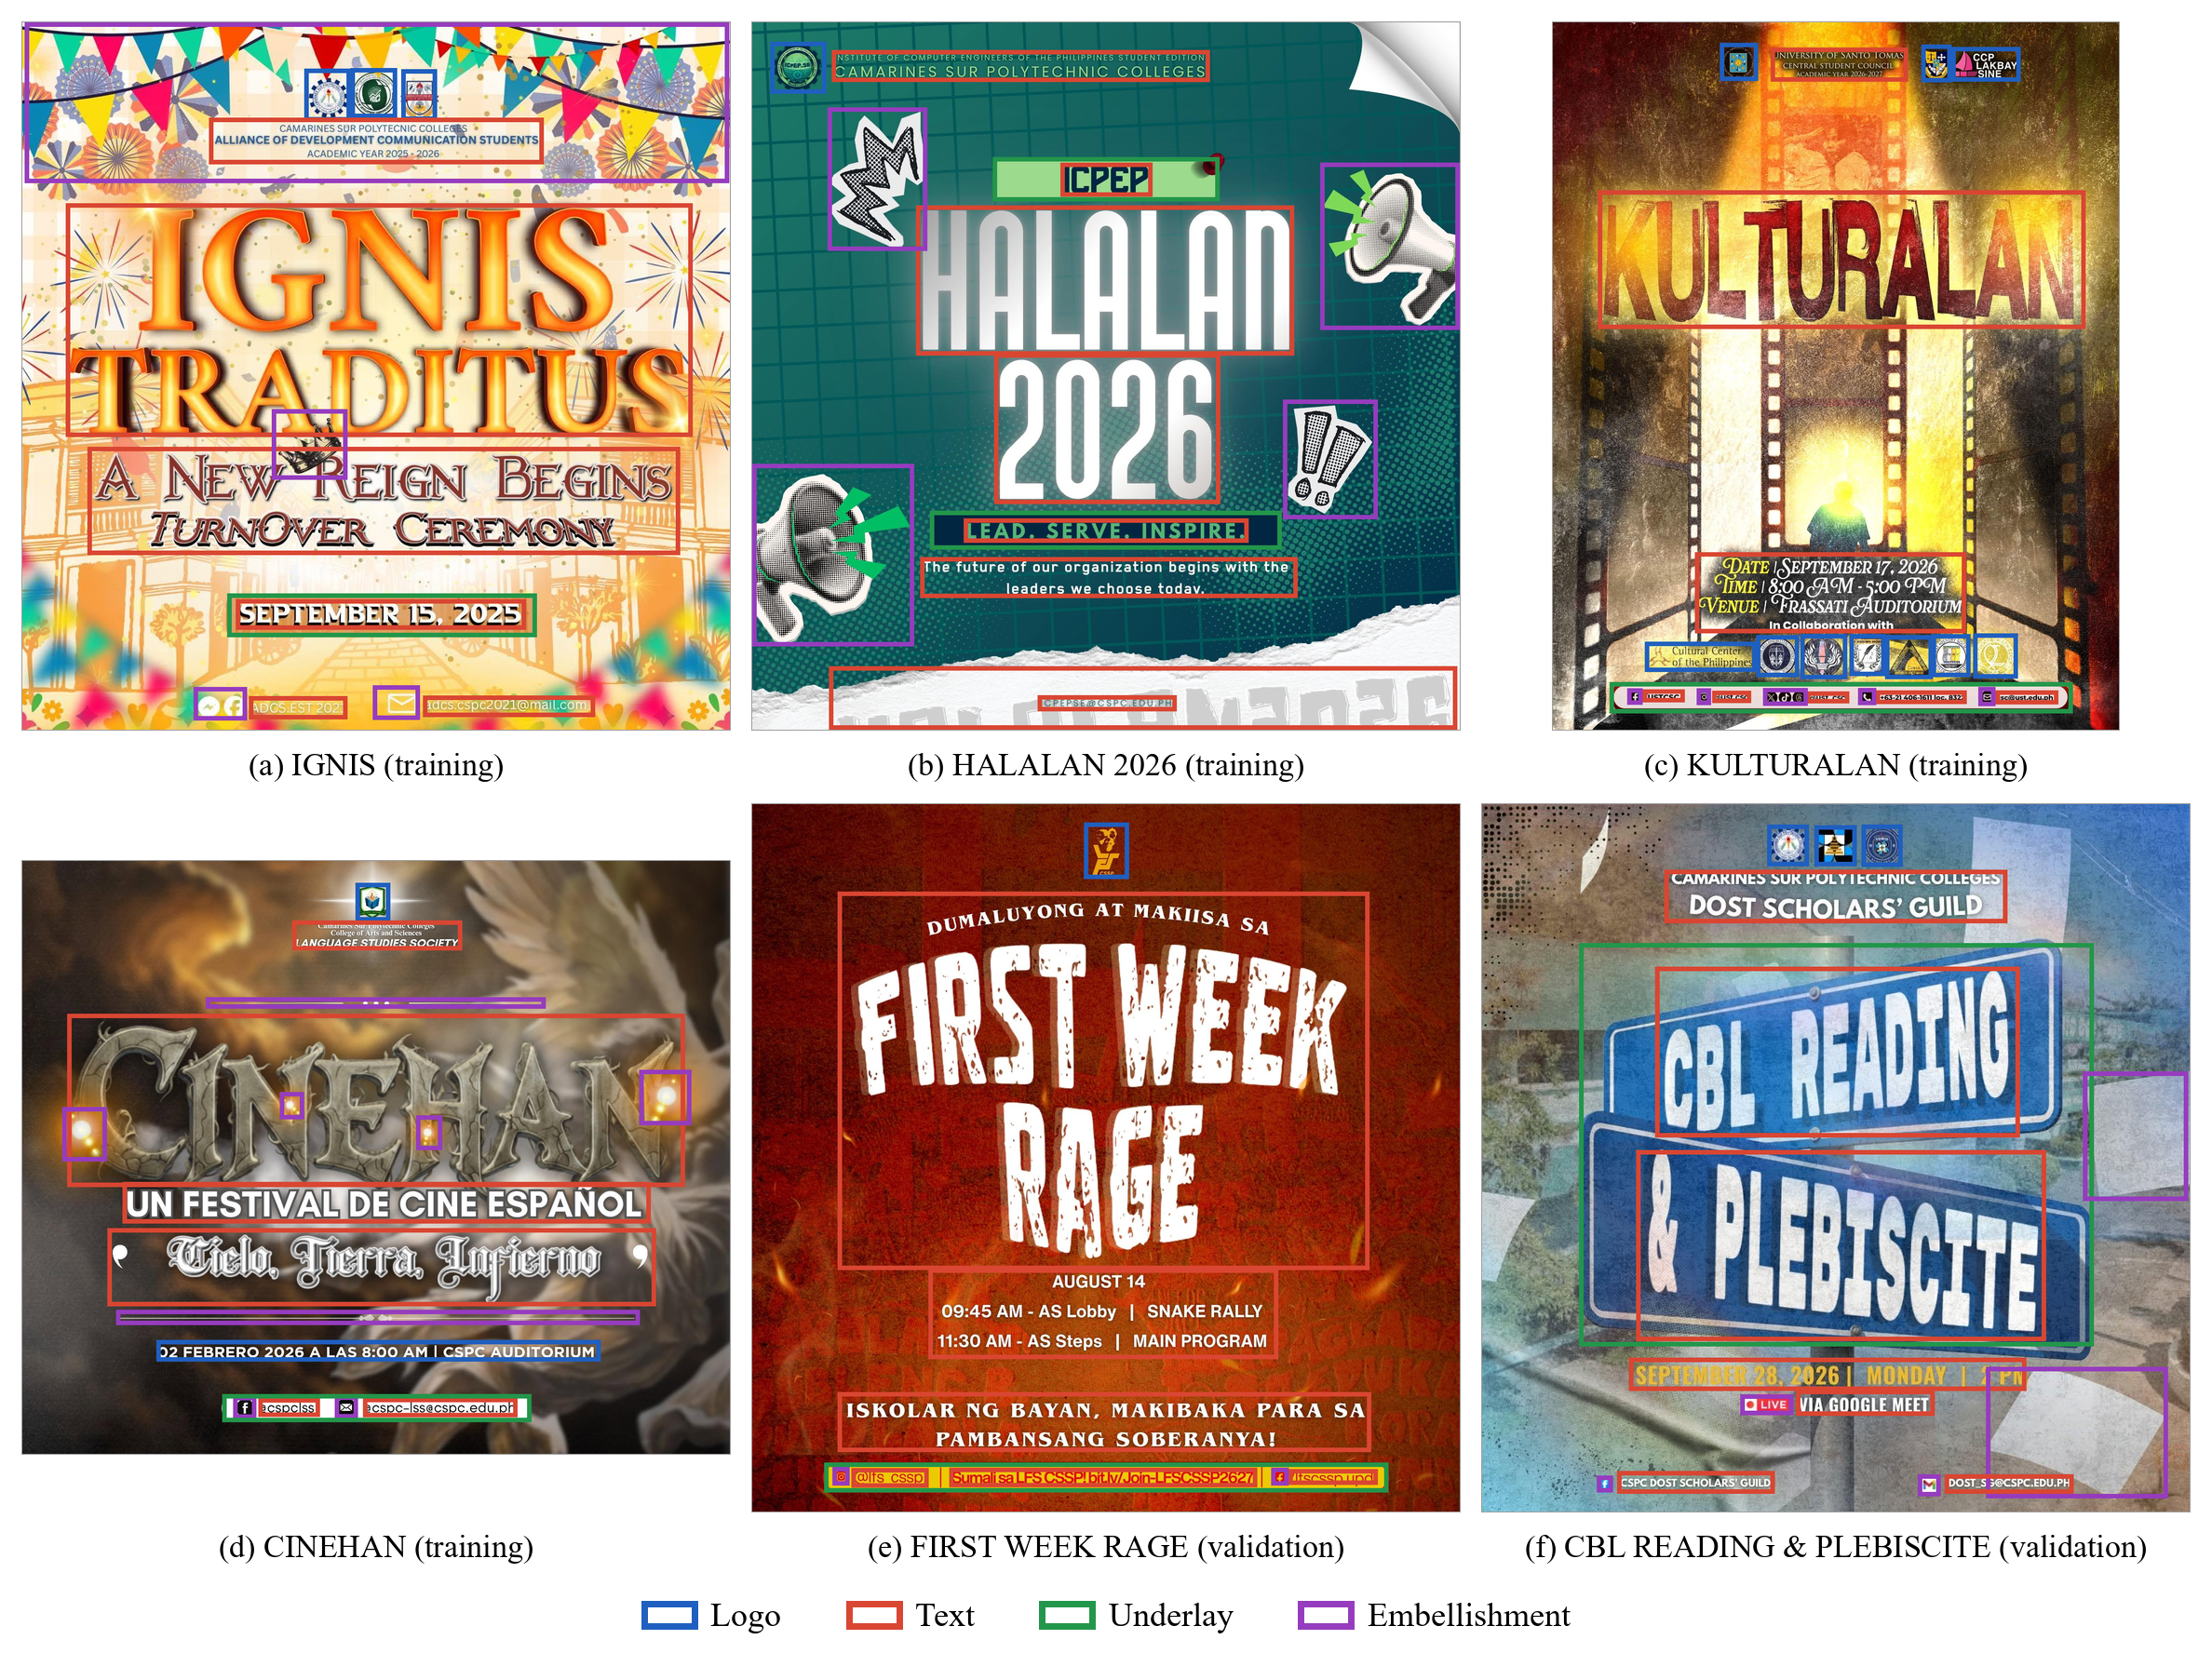
\includegraphics[width=0.66\textwidth]{figures/appendix_c_samples}
    \caption{Sample Annotated Master Layouts From the Empirical Dataset}
    \label{fig:empirical-samples}
\end{figure}
% Drawn from data/raw/master_layout_batch (Roboflow export, version 3) by the manuscript chat's
% appendix_c_figure.py; boxes over 50% of the canvas are left out, as in the training pipeline.

\begin{table}[!ht]
\centering
\caption{Annotated Boxes in the Empirical Dataset by Class}
\label{tab:empirical-counts}
\begin{tabular}{l c c c}
\hline
\textbf{Class} & \textbf{Training (160 images)} & \textbf{Validation (40 images)} & \textbf{Total} \\ \hline
Logo & 544 & 140 & 684 \\
Text & 1,053 & 260 & 1,313 \\
Underlay & 175 & 41 & 216 \\
Embellishment & 740 & 166 & 906 \\ \hline
\textbf{All} & \textbf{2,512} & \textbf{607} & \textbf{3,119} \\ \hline
\multicolumn{4}{p{0.86\textwidth}}{\footnotesize Counts after boxes covering more than 50\% of the canvas were removed (18 in training, 3 in validation). The validation counts are those of \ref{tab:iou}.}
\end{tabular}
\end{table}


\end{theappendices}